\documentclass{standalone}
\usepackage{tikz}
\usetikzlibrary{patterns, positioning}
\usetikzlibrary{shapes.misc}
\usepackage[outline]{contour}
\contourlength{1.5pt} 


\begin{document}
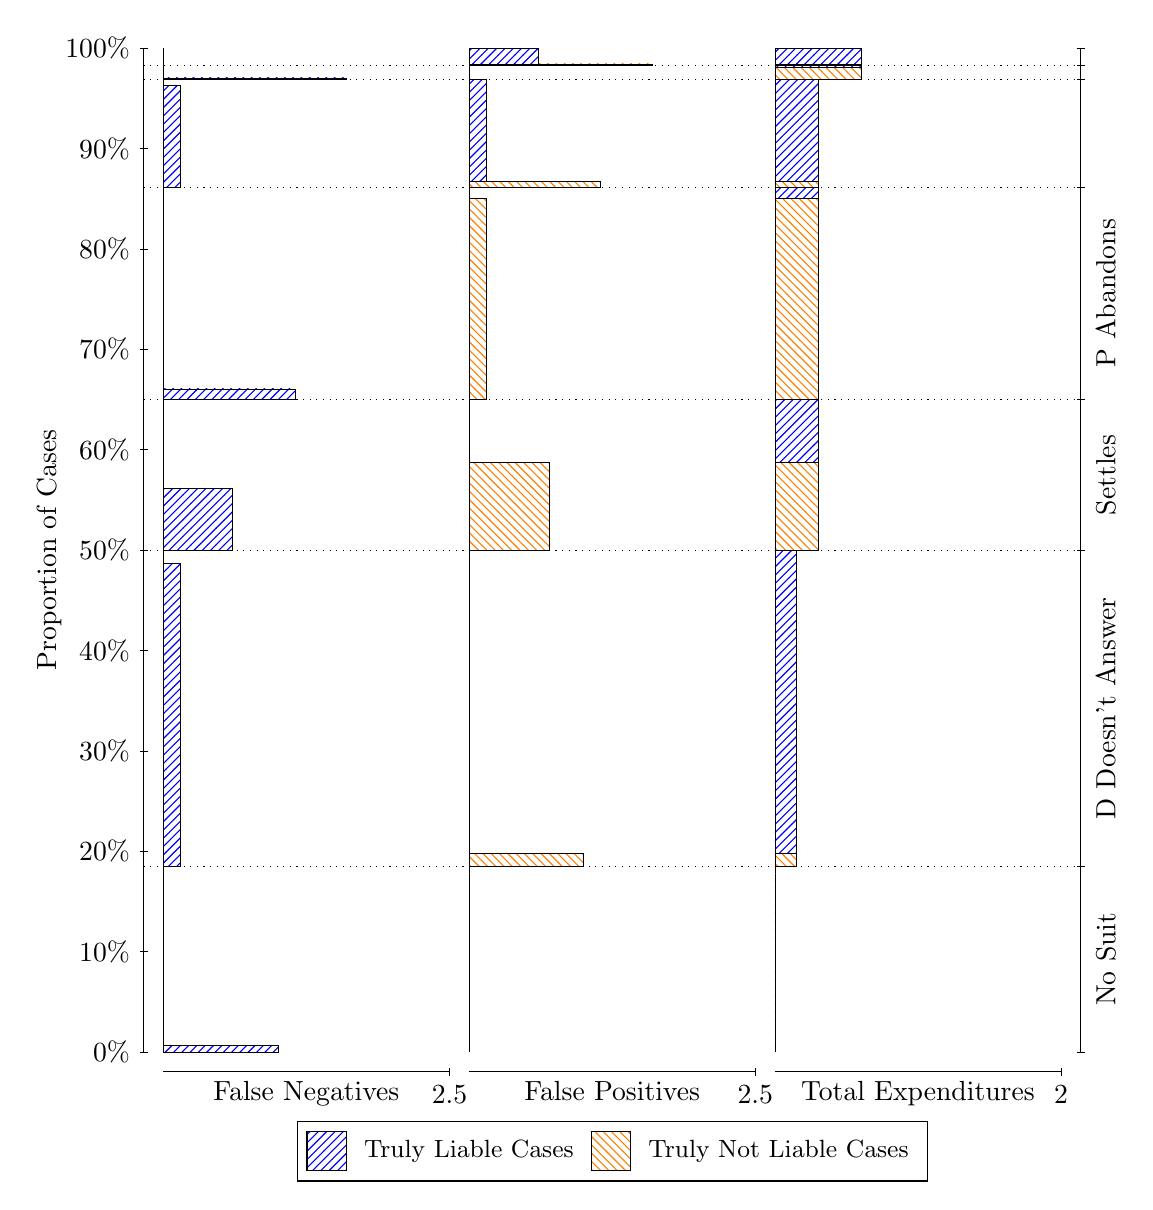
\begin{tikzpicture}
\draw[black, very thin] (1.5,1.75) -- (1.5,14.5);
\node[rotate=90, text=black, anchor=center] at (0.3, 8.125) {Proportion of Cases};
\draw[black, very thin] (1.45,1.75) -- (1.55,1.75);
\node[text=black, anchor=east] at (1.45, 1.75) {0\%};
\draw[black, very thin] (1.45,3.025) -- (1.55,3.025);
\node[text=black, anchor=east] at (1.45, 3.025) {10\%};
\draw[black, very thin] (1.45,4.3) -- (1.55,4.3);
\node[text=black, anchor=east] at (1.45, 4.3) {20\%};
\draw[black, very thin] (1.45,5.575) -- (1.55,5.575);
\node[text=black, anchor=east] at (1.45, 5.575) {30\%};
\draw[black, very thin] (1.45,6.85) -- (1.55,6.85);
\node[text=black, anchor=east] at (1.45, 6.85) {40\%};
\draw[black, very thin] (1.45,8.125) -- (1.55,8.125);
\node[text=black, anchor=east] at (1.45, 8.125) {50\%};
\draw[black, very thin] (1.45,9.4) -- (1.55,9.4);
\node[text=black, anchor=east] at (1.45, 9.4) {60\%};
\draw[black, very thin] (1.45,10.675) -- (1.55,10.675);
\node[text=black, anchor=east] at (1.45, 10.675) {70\%};
\draw[black, very thin] (1.45,11.95) -- (1.55,11.95);
\node[text=black, anchor=east] at (1.45, 11.95) {80\%};
\draw[black, very thin] (1.45,13.225) -- (1.55,13.225);
\node[text=black, anchor=east] at (1.45, 13.225) {90\%};
\draw[black, very thin] (1.45,14.5) -- (1.55,14.5);
\node[text=black, anchor=east] at (1.45, 14.5) {100\%};

\draw[black, very thin] (13.4,1.75) -- (13.4,14.5);
\draw[black, very thin] (13.35,1.75) -- (13.45,1.75);
\node[anchor=west] at (13.35, 1.75) {};
\draw[black, very thin] (13.35,4.1048) -- (13.45,4.1048);
\node[anchor=west] at (13.35, 4.1048) {};
\draw[black, very thin] (13.35,8.1201) -- (13.45,8.1201);
\node[anchor=west] at (13.35, 8.1201) {};
\draw[black, very thin] (13.35,10.033) -- (13.45,10.033);
\node[anchor=west] at (13.35, 10.033) {};
\draw[black, very thin] (13.35,12.733) -- (13.45,12.733);
\node[anchor=west] at (13.35, 12.733) {};
\draw[black, very thin] (13.35,14.1) -- (13.45,14.1);
\node[anchor=west] at (13.35, 14.1) {};
\draw[black, very thin] (13.35,14.28) -- (13.45,14.28);
\node[anchor=west] at (13.35, 14.28) {};
\draw[black, very thin] (13.35,14.5) -- (13.45,14.5);
\node[anchor=west] at (13.35, 14.5) {};

\draw[black, very thin, pattern color=blue, pattern=north east lines] (1.75,1.75) rectangle (3.2033,1.8357);
\draw[black, very thin, pattern color=orange, pattern=north west lines] (1.75,1.8357) rectangle (1.75,4.1048);
\draw[black, very thin, pattern color=blue, pattern=north east lines] (1.75,4.1048) rectangle (1.968,7.9505);
\draw[black, very thin, pattern color=orange, pattern=north west lines] (1.75,7.9505) rectangle (1.75,8.1201);
\draw[black, very thin, pattern color=blue, pattern=north east lines] (1.75,8.1201) rectangle (2.622,8.9113);
\draw[black, very thin, pattern color=orange, pattern=north west lines] (1.75,8.9113) rectangle (1.75,10.033);
\draw[black, very thin, pattern color=blue, pattern=north east lines] (1.75,10.033) rectangle (3.4213,10.171);
\draw[black, very thin, pattern color=orange, pattern=north west lines] (1.75,10.171) rectangle (1.75,12.733);
\draw[black, very thin, pattern color=blue, pattern=north east lines] (1.75,12.733) rectangle (1.968,14.023);
\draw[black, very thin, pattern color=orange, pattern=north west lines] (1.75,14.023) rectangle (1.75,14.1);
\draw[black, very thin, pattern color=blue, pattern=north east lines] (1.75,14.1) rectangle (4.0753,14.122);
\draw[black, very thin, pattern color=orange, pattern=north west lines] (1.75,14.122) rectangle (1.75,14.28);
\draw[black, very thin, pattern color=orange, pattern=north west lines] (1.75,14.28) rectangle (1.75,14.298);
\draw[black, very thin, pattern color=blue, pattern=north east lines] (1.75,14.298) rectangle (1.75,14.5);
\draw[black, very thin, pattern color=orange, pattern=north west lines] (5.6333,1.75) rectangle (5.6333,4.0191);
\draw[black, very thin, pattern color=blue, pattern=north east lines] (5.6333,4.0191) rectangle (5.6333,4.1048);
\draw[black, very thin, pattern color=orange, pattern=north west lines] (5.6333,4.1048) rectangle (7.0867,4.2745);
\draw[black, very thin, pattern color=blue, pattern=north east lines] (5.6333,4.2745) rectangle (5.6333,8.1201);
\draw[black, very thin, pattern color=orange, pattern=north west lines] (5.6333,8.1201) rectangle (6.6507,9.2423);
\draw[black, very thin, pattern color=blue, pattern=north east lines] (5.6333,9.2423) rectangle (5.6333,10.033);
\draw[black, very thin, pattern color=orange, pattern=north west lines] (5.6333,10.033) rectangle (5.8513,12.595);
\draw[black, very thin, pattern color=blue, pattern=north east lines] (5.6333,12.595) rectangle (5.6333,12.733);
\draw[black, very thin, pattern color=orange, pattern=north west lines] (5.6333,12.733) rectangle (7.3047,12.81);
\draw[black, very thin, pattern color=blue, pattern=north east lines] (5.6333,12.81) rectangle (5.8513,14.1);
\draw[black, very thin, pattern color=orange, pattern=north west lines] (5.6333,14.1) rectangle (5.6333,14.257);
\draw[black, very thin, pattern color=blue, pattern=north east lines] (5.6333,14.257) rectangle (5.6333,14.28);
\draw[black, very thin, pattern color=orange, pattern=north west lines] (5.6333,14.28) rectangle (7.9587,14.298);
\draw[black, very thin, pattern color=blue, pattern=north east lines] (5.6333,14.298) rectangle (6.5053,14.5);
\draw[black, very thin, pattern color=orange, pattern=north west lines] (9.5167,1.75) rectangle (9.5167,4.0191);
\draw[black, very thin, pattern color=blue, pattern=north east lines] (9.5167,4.0191) rectangle (9.5167,4.1048);
\draw[black, very thin, pattern color=orange, pattern=north west lines] (9.5167,4.1048) rectangle (9.7892,4.2745);
\draw[black, very thin, pattern color=blue, pattern=north east lines] (9.5167,4.2745) rectangle (9.7892,8.1201);
\draw[black, very thin, pattern color=orange, pattern=north west lines] (9.5167,8.1201) rectangle (10.062,9.2423);
\draw[black, very thin, pattern color=blue, pattern=north east lines] (9.5167,9.2423) rectangle (10.062,10.033);
\draw[black, very thin, pattern color=orange, pattern=north west lines] (9.5167,10.033) rectangle (10.062,12.595);
\draw[black, very thin, pattern color=blue, pattern=north east lines] (9.5167,12.595) rectangle (10.062,12.733);
\draw[black, very thin, pattern color=orange, pattern=north west lines] (9.5167,12.733) rectangle (10.062,12.81);
\draw[black, very thin, pattern color=blue, pattern=north east lines] (9.5167,12.81) rectangle (10.062,14.1);
\draw[black, very thin, pattern color=orange, pattern=north west lines] (9.5167,14.1) rectangle (10.607,14.257);
\draw[black, very thin, pattern color=blue, pattern=north east lines] (9.5167,14.257) rectangle (10.607,14.28);
\draw[black, very thin, pattern color=orange, pattern=north west lines] (9.5167,14.28) rectangle (10.607,14.298);
\draw[black, very thin, pattern color=blue, pattern=north east lines] (9.5167,14.298) rectangle (10.607,14.5);
\draw[black, dotted] (1.5,4.1048) -- (13.4,4.1048);
\draw[black, dotted] (1.5,8.1201) -- (13.4,8.1201);
\draw[black, dotted] (1.5,10.033) -- (13.4,10.033);
\draw[black, dotted] (1.5,12.733) -- (13.4,12.733);
\draw[black, dotted] (1.5,14.1) -- (13.4,14.1);
\draw[black, dotted] (1.5,14.28) -- (13.4,14.28);
\draw[black, very thin] (1.75,1.5) -- (5.3833,1.5);
\node[text=black, anchor=north] at (3.5667, 1.5) {False Negatives};
\draw[black, very thin] (5.3833,1.45) -- (5.3833,1.55);
\node[text=black, anchor=north] at (5.3833, 1.45) {2.5};

\draw[black, very thin] (5.6333,1.5) -- (9.2667,1.5);
\node[text=black, anchor=north] at (7.45, 1.5) {False Positives};
\draw[black, very thin] (9.2667,1.45) -- (9.2667,1.55);
\node[text=black, anchor=north] at (9.2667, 1.45) {2.5};

\draw[black, very thin] (9.5167,1.5) -- (13.15,1.5);
\node[text=black, anchor=north] at (11.333, 1.5) {Total Expenditures};
\draw[black, very thin] (13.15,1.45) -- (13.15,1.55);
\node[text=black, anchor=north] at (13.15, 1.45) {2};

\node[text=black, centered, rotate=90] at (13.72, 2.9274) {\contour{white}{No Suit}};
\node[text=black, centered, rotate=90] at (13.72, 6.1125) {\contour{white}{D Doesn't Answer}};
\node[text=black, centered, rotate=90] at (13.72, 9.0768) {\contour{white}{Settles}};
\node[text=black, centered, rotate=90] at (13.72, 11.383) {\contour{white}{P Abandons}};




\draw (7.449999999999999,1.5) node[draw=none] (baseCoordinate) {};
\begin{scope}[align=center]
        \matrix[scale=0.5, draw=black, below=0.5cm of baseCoordinate, nodes={draw}, column sep=0.1cm]{
            \node[rectangle, draw, minimum width=0.5cm, minimum height=0.5cm, pattern color=blue, pattern=north east lines] {}; &
            \node[draw=none, font=\small, text=black] (B) {Truly Liable Cases}; &
            \node[rectangle, draw, minimum width=0.5cm, minimum height=0.5cm, pattern color=orange, pattern=north west lines] {}; &
            \node[draw=none, font=\small, text=black] (B) {Truly Not Liable Cases}; \\
            };
\end{scope}

\end{tikzpicture}
\end{document}